\chapter{State of the Art} \label{ch:sota}
This chapter discusses the current state of the art in the fields of Gradient Based Explanations and Augmentations for CNNs. The chapter is divided into two sections, one for each of the fields. The first section discusses the various methods used to explain the predictions of CNNs. The second section discusses the various methods used to augment the training data for CNNs. This chapter also discusses the limitations of the current methods and the motivation behind Proxy Attention.

\section{Gradient Based Explanations} \label{sec:gradient_based_explanations}
\textcolor{red}{Need for Explanations}
% 1. **Interpretability**: Providing explanations for the predictions made by deep learning models is crucial in making these models interpretable. This helps in understanding the decision-making process of the models and promotes trust among stakeholders.

% 2. **Debugging**: Explaining the output of a deep learning model can be beneficial for debugging purposes. If a model makes an unexpected prediction, inspecting the explanation can help identify what went wrong.

% 3. **Fairness**: Explainability can help ensure fairness by allowing us to see if the model is using inappropriate features to make its decisions, such as race, gender, or other protected characteristics. 

% 4. **Safety**: In safety-critical systems such as self-driving cars or medical diagnosis, it's important to understand why the system made a certain decision. Explainability can provide insights into these decisions and help prevent potentially harmful outcomes.

% 5. **Regulatory compliance**: Some regulations require decisions made by AI systems to be explainable. GDPR, for instance, includes a "right to explanation" of automated decisions.

% 6. **Trust**: If a system can explain its actions in a way that humans understand, it is more likely to be trusted by the users. 

% 7. **Robustness**: Understanding a model's decision-making process can lead to designing more robust models, as it allows us to uncover the model's weak spots.

% 8. **Ethics**: Explainability can help ensure that the AI is behaving ethically, by providing transparency into the factors driving its decisions.

% 9. **Education**: Explainability can help non-experts learn more about how a complex system works, and can make it easier to teach machine learning concepts.

% 10. **Generalization**: By understanding why a model makes certain decisions, we can determine if it is generalizing well to new data, or if it is merely overfitting to the training data.

% 11. **Bias detection**: Explainability can be used to detect and mitigate any bias in the decisions made by the AI, leading to fairer outcomes.

% 12. **Feature Importance**: It helps in determining which features are important for making predictions, providing insights about the problem space.

% 13. **User Experience**: Explainability can improve the user experience by making the AI's outputs more understandable and relatable.

% 14. **Model Improvement**: Explainability can lead to model improvement. Once we understand why a model is making certain mistakes, we can try to adjust the model or the data it is trained on to correct these issues.

% 15. **Model Selection**: When comparing multiple models, explainability can assist in selecting the model that not only performs well but also makes decisions in a way that aligns with human understanding or domain knowledge.

% Deconvnet
One of the earlier approaches to Saliency maps for CNNs was proposed by Zeiler et al. \cite{zeilerVisualizingUnderstandingConvolutional2013} termed DeconvNet. DeconvNet works by inverting the network's operations in the forward pass. After attaching the DeconvNet layers to the network, propagating through these layers represents features that the original CNN possessed. The relevant reconstruction can be obtained for a single class by setting all the activations other than the one corresponding to the class to zero. The resulting image is then used to generate the saliency map. A Deconv layer replaces the Conv layer, and the ReLU operation has negative values clamped. While the pooling operation is not strictly invertible, the authors use switch variables that store the maximum value position for each pooling operation. While the DeconvNet works to a certain extent, the results are less accurate than the ones obtained by other methods and are also biased towards the representations of the first layer.

% Deep Inside Conv Nets
Building on the DeconvNet, Simonyan et al. \cite{simonyanDeepConvolutionalNetworks2014} extrapolate the idea of class visualization to create one of the first approaches to Saliency maps. Their approach, also called Vanilla Gradient, ranks the pixels of an image $I_{0}$ by how important they are in the prediction of the Saliency score $S_{c}(I) \approx w^{T}I + b$. In this equation, $w$ and $b$ are the network weights and biases obtained by back-propagating wrt the image itself. The objective to be minimized thus is $arg \underset{I}max S_{c}(I) - \lambda||I||^{2}_{2}$ where $\lambda$ is used as a regularization parameter. Using these equations, a saliency map $A \in \mathbb{R}^{m \times n}$ ($m \times n$ stands for $height \times width$) can be computed. To find the map, we find the derivative of $w$, rearrange the elements and then process them according to the number of input channels. If the number of channels is greater than one, the maximum value over the channel is considered $A_{i,j}= \underset{ch}max |w_{h_{(i,j, ch)}}|$. Where $ch$ is the colour channel of the pixel $(i,j)$, $h(i,j, ch)$ is the index of the $w$ corresponding to that pixel. The Vanilla Gradient method produces an approximate saliency map but has much noise. This leads to issues for more complex images. The methods proposed in the following papers have addressed many of the issues with Vanilla Gradients and DeconvNets \cite{zeilerVisualizingUnderstandingConvolutional2013}.

% Scorecam
In another paper, the authors propose a score-weighted approach - ScoreCAM to create saliency maps \cite{wangScoreCAMScoreWeightedVisual2020}. Like many other methods, the images are first passed through the network, and the corresponding activations are obtained from the final convolutional layer. These activation maps are upsampled and normalized to $[0,1]$. The highlighted activation map portions are then passed through a CNN with a SoftMax layer to obtain the score for each of the current classes. These scores are used to find the activation maps' relative importance. Finally, the sum of all these maps is computed using a linear combination with the corresponding target score and then passed through a ReLU operation. These operations can be mathematically represented as $L^{c}_{ScoreCAM} = ReLU(\underset{k}\Sigma w_{k}^{c}A^{k})$, where $k$ represents the index considered, $c$ represents the current class and $S_k$ represents the outputs of the SoftMax as mentioned earlier layer. The authors find that the maps obtained using ScoreCAM are less noisy, and this method removes the dependency on unstable gradients compared to other methods.

% Guided Gradcam
A variant of GradCAM \cite{selvarajuGradCAMVisualExplanations} was proposed by Selvaraju et al. \cite{selvarajuGradCAMWhyDid2017} where, unlike GradCAM that finds the parts of the image that influence the model's decision, Guided GradCAM takes the positive gradients into account. These gradients are used to obtain an even more fine-grained representation of the outputs of the saliency map. While GradCAM backpropagates both positive and negative gradients, Guided Backprop only propagates the positive gradients and is defined as a pointwise multiplication of the results of GradCAM and Guided Backpropagation \cite{springenbergStrivingSimplicityAll2015}.

% Noise Tunnel
In combination with attribution methods, Noise Tunnel \cite{kokhlikyanCaptumUnifiedGeneric2020} is an algorithm that improves the accuracy of the masks obtained by these methods. Noise Tunnel was proposed to counter noisy and irrelevant attributions obtained by some gradient-based methods by adding a Gaussian Noise and then averaging the predictions over sampled attributions. Since all the samples are considered, this method has a significant computational overhead. For Smooth Grad \cite{smilkovSmoothGradRemovingNoise2017}, the new attribution is defined as $\hat M_{c}(x) = \frac{1}{n}\Sigma_{1}^{n}M_{c}(x + \mathcal{N}(0, \sigma^{2}))$. Where $M_{c}$ is the attribution calculated by SmoothGrad, $\mathcal {N}(0, 0.01^2)$ is the Gaussian Noise with $\sigma = 0.01$ and $n$ is the number of samples. Similarly for Smooth Grad Square, $\hat M_{c}(x) = \frac{1}{n}\Sigma_{1}^{n}\sqrt{M_{c}(x + \mathcal{N}(0, \sigma^{2}))}$. Noise Tunnel can also be used on Var Grad \cite{richterVarGradLowVarianceGradient2020} with the equation $\hat M_{c}(x) = \frac{1}{n}\Sigma_{k=1}^{n}\{M_{c}(x + \mathcal{N}(0, \sigma^{2}))\}^{2}- \{\hat M_{c}(x)\}^{2}$

% Integrated Gradients
For a model $F$, the attribution method Integrated Gradients \cite{sundararajanAxiomaticAttributionDeep2017} computes the contribution of each pixel in the image towards the final prediction. The model's output is used to calculate a pixel-wise partial derivative that is then integrated along a path starting from the baseline and ending at the input. Each step is scaled according to the partial derivative obtained in the previous step. For every step k with m total steps over the path, the IG equation is defined as $IntegratedGrads_i^{approx}(x)::=(x_{i}-x_i')\times \Sigma_{k=1}^{m}\frac{\partial F(x' + \frac{k}{m} \times (x-x'))}{\partial x_{i}} \times \frac{1}{m}$. Where $(x_{i} - x_{i}')$ is the pixel-wise difference between the two images, $\frac{\partial F(x' + \frac{k}{m} \times (x-x'))}{\partial x_i}$ is the partial derivative of the model output $F$ with respect to pixel $i$ at the $k$-th step of the path, and $\frac{1}{m}$ is the scaling factor that ensures that each of the steps taken contributes equally to the final result.

% Rise
Petsiuk et al. propose RISE \cite{petsiukRISERandomizedInput2018}, a saliency method that randomly alters the input images by applying random noise to each. After model predictions are obtained, the saliency map is generated by combining the partial maps over each modified image. RISE improves accuracy but needs a lot of computation time, considering that multiple models must be trained for each random noise sample.

% Influence Of Image Class Acc On Saliency Map Estimation
Oyama et al. \cite{oyamaInfluenceImageClassification2018} found a strong correlation concerning the relationship between saliency maps and image classification accuracy. The authors found that the architecture and the initialization strategy influence the final saliency map. By analyzing the generated saliency maps, they find that if the model is randomly initialized and trained for image classification, having limited categories in the original dataset leads to overfitting. On the other hand, having many categories suppresses the overfitting of the objects present in the training dataset. On training their proposed network ReadoutNet on a fixation task (which requires the network to learn where to focus), they found that the accuracy of estimating the saliency map was linked to the image classification accuracy.

% Summit
While a large amount of research focuses on interpreting the influence of a single image or neuron, Hohman et al. propose Summit, \cite{hohmanSummitScalingDeep2019} a novel scalable summarization algorithm. Summit creates an attribution graph that distils the influence of neurons and substructures throughout the network used to make the final prediction. The attribution graph is created due to combining activation aggregation, a technique to find important neurons and neuron-influence aggregation, a technique to find relationships among the neurons identified in the previous step. After a forward pass through the network, the activation channels maximums are obtained to aggregate the activations. These are then filtered by class and aggregated by taking the top $k$ channels or the top $k$ channels by weight. To quantify how much a layer influences the next, the authors aggregate the influences by creating a tensor $I^{l}$ for all the network layers ($l$). How important channel $i$ of the layer $l-1$ is determined by the aggregate tensor $I^{l}_{cij}$ where $j$ represents the output channel and $c$ is the class of the image. Considering the $j^{th}$ kernel of the layer $K^{(j)} \in \mathbb{R}^{H \times W \times C_{l-1}}$, a single channel $Y$ can be represented using the 3D convolution operation by $Y_{:,:,j}= X \ast K^{(j)}$. This is equivalent to it's representation by the 2D convolution $Y_{:,:,j}= \Sigma_{i=1}^{C_{l-1}} X_{:,:,i} \ast K^{(j)}_{:,:,i}$. The value $X_{:,:,i} \ast K^{(j)}_{:,:,i}$ is the contribution of the current channel from the previous layer and the maximum of this value is used to generate the influence map.

% Conductance
Building upon Integrated Gradients, Dhamdhere et al. propose \cite{dhamdhereHowImportantNeuron2018} Conductance, a means to boost the attributions provided by IG to specific neurons in the hidden layer. This is done by decomposing the computation that IG performs. The authors apply this method to the Inception network \cite{szegedyGoingDeeperConvolutions2014} and can find the filters that influence the final predictions most. 
For a neuron $y$ , the network can be represented as a function $F:R^{n} \rightarrow [0,1]$. Given an input $x \in R^{n}$ and a baseline input $x' \in R^{n}$, the IG for the $i^{th}$ dimension at $x$ is given by $IG_{i}(x) ::== (x_{i}- x_{i}') \int_{\alpha=0}^{1} \frac{\partial F(x' + \alpha(x-x'))}{\partial x_{i}}d \alpha$ . Considering $\frac{\partial F(x)}{\partial x_{i}}$ to be the gradient of $F$ along $i^{th}$ dimension at x, the Conductance for $y$ can be defined as $
Cond_{i}^{y}(x) ::== (x_{i}- x_{i}') \int_{\alpha=0}^{1} \frac{\partial F(x' + \alpha(x-x'))}{\partial y} \cdot \frac{\partial y}{\partial x_{i}} d \alpha$. The authors also propose methods of evaluating Conductance by the assumption that an influential hidden network should be good at predicting the given input class. This assumption can be validated by two metrics : the $Gradient\times Activation$ : $
y \times \frac{\partial F(x' + \alpha \times (x-x'))}{\partial y} d \alpha$ and the Internal Influence : $
IntInf ^{y}(x) ::= \int^{1}_{\alpha=0} \frac{\partial F(x' + \alpha(x-x'))}{\partial y} d \alpha$.\\

% Smooth Grad
Consider an image classification task where an input image $x$ is classified as a single class from a set $C$. For every class $c \in C$, the output class is represented as $class(x) = argmax_{c \in C}S_{c}(x)$. Using this $class$, a sensitivity map $M_{c}(x)$ can be generated by differentiating with respect to $x$, $M_{c}(x) = \frac{\partial S_{c}}{\partial x}$ . $M_{c}$, being a sensitivity map (\cite{simonyanDeepConvolutionalNetworks2014}), thus representing the influential regions of the image used to make the prediction. Since these maps are noisy, Smilkov et al. propose SmoothGrad \cite{smilkovSmoothGradRemovingNoise2017}, a modification of the previous method where instead of using $\partial S_{c}$, a smoothing is applied using a Gaussian kernel to $\partial S_{c}$. The authors also find that it is impossible to directly compute the smoothing due to high dimensionality and thus approximate the calculation by averaging multiple maps computed in the neighbourhood of $x$ using random sampling. The final SmoothGrad equation then becomes $\hat M_{c}(x) = \frac{1}{n}\Sigma_{1}^{n}M_{c}(x + \mathcal{N}(0, \sigma^{2}))$, where $\mathcal{N}(0, \sigma^{2})$ is the Gaussian noise and $\sigma$ is the standard deviation.

% \textcolor{red}{Deep Lift}
% Deep Visual Explanations
The ability of a model to explain the reason for it's predictions in the context of an image classification task is known as Deep Visual Explanation (DVE). Babiker et al. \cite{babikerIntroductionDeepVisual2018} propose a method to generate DVEs by using the activation of different spatial scales in the Fourier space. Since CNNs generate spatial information at different layers, the authors use this information in the form of feature maps to generate explanations. The activations that do not contribute to the final prediction are penalized and the final explanation is generated by combining the activations of the high and low spatial scales in the aforementioned Fourier space. Combining the explanations provided by these two scales allows the authors to generate a more targeted explanation.

% Embedding Knowledge Into Deep Attention Map
Mitsuhara et al. \cite{mitsuharaEmbeddingHumanKnowledge2019} propose an approach that involves manually editing the attention maps generated by the network to provide the model with expert human input. They use an Attention Branch Network (ABN), fine tune it using the manually edited attention maps and then use the fine tuned model to generate the final attention map. The authors also demonstrate a tool that can be used to interactively modify the attention maps using a mouse. This tool takes misclassified images as input and allows the user to add or remove attention regions before passing the edited attention map to the network. The authors also demonstrate that the fine tuned model performs better than the original model due to the additional expert input.

% Sam Resnet
Another approach to creating attention maps involves using an LSTM \cite{corniaPredictingHumanEye2018} (SAM). The authors use a ResNet to extract feature maps from the input image, which are then passed to an Attentive Convolutional LSTM for refinement. A separate module is used to add priors to the attention map to account for the center bias present in human eye fixations. Many advantages that LSTMs provide are used in the research, such as the ability to process features in an iterative way. The attention map is generated with a convolution of the previous hidden state and the input, which is then normalized using the softmax operator. The authors find that the attention maps generated by SAM are quite accurate and using a modified version of the ResNet, they are able to generate attention maps that are of higher resolution.

\textcolor{red}{CAM}

\textcolor{red}{Gradcam++}

\textcolor{red}{Guided Backprop}

\textcolor{red}{Salience Map}

\section{Augmentation} \label{sec:augmentation}
\textcolor{red}{Need for Augmentation}
% - sufficient open datasets like Imagenet [Russakovsky et al., 2015], MS-COCO [Lin et al., 2014] and PASCAL VOC [Everingham et al., 2015] are crucial to the development of deep learning models. 
% - - The core idea of data augmentation is to improve the sufficiency and diversity of training data by generating synthetic dataset 
% - The augmented data can be regarded as being extracted from a distribution that is close to the real one 
% - augmented dataset can represent more comprehensive characteristics 
% - data augmentation methods are tasks-independent 
% - Because the operations are performed on the image data and labels at the same time, and the label types are different under different tasks, the data augmentation methods for object detection task can not be directly applied to semantic segmentation task  
% - [[Image Erasing]]
% - delete one or more sub-regions in the image 
% - replace the pixel values of these sub-regions with constant values or random values 
% - Hide-and-Seek 
% - random erasing 
% - GridMask 
% - Cutout 
% - FenceMask 
% - simulation of object occ

% - [[Image Mix]]
% - mixing two or more images or sub-regions of images into one. 
% - mixup

% - [[Image Manipulation]]
% - image transformations, such as rotation, flipping, and cropping, etc 
% - manipulate the images directly and are easy to implement 
% - CutMix 
% - [[Fmix]]
% - AugMix 
% - [[ManifoldMix]]

% - [[Auto Augment]]
% - search algorithm and search space 
% - The search algorithm is designed to find the best policy regarding highest validation accuracy 
% - The search space contains many policies which details various augmentation operations and magnitudes with which the operations are applied 
% - [[Fast AutoAugment]]
% - [[Population Based Augmentation]]
% - [[RandAugment]]


% - [[Feature Augmentation]]
% - Rather than conduct augmentation only in the input space, feature augmentation performs the transformation in a learned feature space 
% - [DeVries and Taylor, 2017a] 
% - when traversing along the manifold it is more likely to encounter realistic samples in feature space than compared to input space 
% - feat match, moment exchange

% - [[Deep Generative Models]]
% - The ultimate goal of data augmentation is to draw samples from the distribution, which represent the generating mechanism of dataset 
% - the data distribution we generate data from should not be different with the original one 
% - StarGAN, pix2pix
\begin{figure}[htbp]
    \centering
    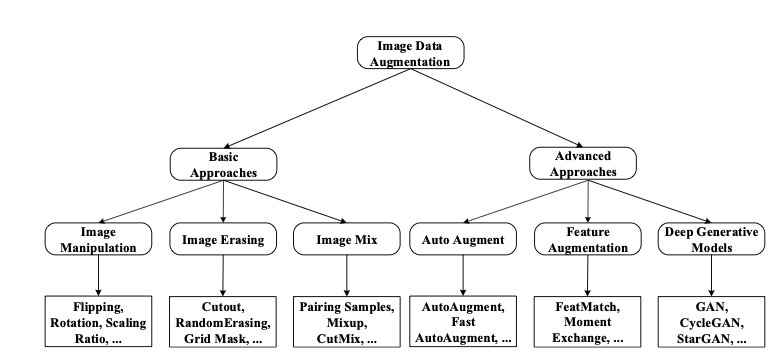
\includegraphics[width=.9\textwidth]{images/data_aug_categories.png}
    \caption{Categories of Data Augmentation (sourced from \cite{yangImageDataAugmentation2022})}
    \label{fig:categorization_augmentation}
\end{figure}

% Augmix
Another augmentation strategy proposed by \cite{hendrycksAugMixSimpleData2020} first applies multiple transformations randomly and in parallel chains to each image. These transformations can include combinations of Translation, Rotation, Shearing and others. The outputs of these combinations are then mixed to form a new image, which is further mixed with the original image to form the new image. This combination improves performance in cases where data shifts are encountered in production. Once the images are mixed, a skip connection is used to combine the results of the chains. AugMix also uses the Jensen-Shannon Divergence consistency loss \cite{linDivergenceMeasuresBased} to ensure the images are stable across various inputs. Considering $KL$ to be Kullback-Leibler Divergence, the Jensen-Shannon Divergence can be defined as $
    JS(p_{orig}; p_{augmix1};p_{augmix2}) = \frac{1}{3}(KL[p_{orig}||M||]+KL[p_{augmix1}||M||]+KL[p_{augmix2}||M||])
$, where $M$ is the mean of the three distributions $p_{orig}, p_{augmix1}, p_{augmix2}$.

% Cutout
Devries et al., in their paper \cite{devriesImprovedRegularizationConvolutional2017}, propose an augmentation method they call Cutout. This method removes random-sized square patches from the images by replacing the corresponding pixels with a constant value (usually 0). Selecting the region involves picking a random pixel value and creating a uniform-sized square around the chosen pixel. The authors also find that Cutout performs better with other methods than just being used by itself. Cutout can be expressed as an element-wise multiplication operation $x_{cutout} = x \odot M$,
$x$ is the original image, $M$ is a binary mask of the same size as $x$ with randomly chosen coordinates of a square patch of pixels to be cut out, and $\odot$ denotes element-wise multiplication.

% Cut and mix
Unlike Cutout \cite{devriesImprovedRegularizationConvolutional2017}, where the chosen patch is replaced with zero pixels, in CutMix \cite{yunCutMixRegularizationStrategy2019}, the chosen patch is replaced with a randomly chosen patch from a different region of the same image. Yun et al. propose this approach as multiple class labels can be learned with a single image.
CutMix can be defined by the following operations $\overset{\sim}x = M \odot x_{A} + (1-M) \odot x_{B}$ ; $\overset{\sim}y = \lambda y_{A}+ (1- \lambda)y_{B}$. $x$ is an RGB image, $y$ is the respective label, $M$ is a binary mask of the image patch that will be dropped, and $\odot$ represents element-wise multiplication. The new training sample $\overset{\sim}x , \overset{\sim}y$ is created by combining two other training samples $x_{A}, y_{A}$ and $x_{B} , y_{B}$. To control the combination ratio $\lambda$, a sample from the $\beta(1,1)$ distribution is chosen. This combination is quite similar to \cite{zhangMixupEmpiricalRisk2018} but differs in the sense that CutMix focuses on generating locally natural images.

% Attentive Cutmix
Building upon \cite{yunCutMixRegularizationStrategy2019}, Walawalkar et al. propose an alternative method of replacing patches in an image they call Attentive CutMix \cite{walawalkarAttentiveCutMixEnhanced2020}. Instead of randomly pasting patches in the image, this method uses a pre-trained network to identify attentive regions from the image. Similar to the earlier approach, these patches are mapped back to the original image. Doing so allows the network to select important background regions for the task while also updating the label information.

% Cow Mask
Many of the algorithms use rectangular or square-shaped masks. While effective, French et al. propose Cow Mask \cite{frenchMilkingCowMaskSemiSupervised2020}, a new masking method that uses irregularly shaped masks with a Gaussian filter to reduce noise. The authors also propose two mixing methods, one that builds up on Random Erasing \cite{zhongRandomErasingData2020}, and another that uses Cut Mix \cite{yunCutMixRegularizationStrategy2019}. A pixel-wise mixing threshold is also chosen, and either mixing or erasing is applied to the image based on this threshold. This augmentation technique is shown to be effective in semi-supervised learning.

% Cut Paste Learn
\ proposed another approach involving a cut-paste methodology cite{dwibediCutPasteLearn2017}. In their paper, the authors propose a new method of augmentation that extracts instances of objects from the images. Instead of pasting them on other images, they are pasted on randomly chosen backgrounds. This method leads to pixel artefacts in the images, as selecting the objects is a noisy process. To overcome the drop in performance, the authors apply a Gaussian blur and Poisson blending to the boundaries of the pasted objects. Further augmentation is applied before pasting the objects by rotation, occlusion and truncation. The authors also find that this approach makes the network more robust to image artefacts.

% Hide and Seek
In their paper, Singh et al. \cite{singhHideandSeekDataAugmentation2018} propose a data augmentation method that takes an image as an input and divides it into a grid. Each of the sub-grids is then turned off with a given probability. These sub-grids can be connected or independent of each other, and the turned-off grids are replaced by the average pixel value of all the images in the dataset.

% GridMask
One of the major drawbacks of algorithms that rely on modifying image patches (such as \cite{singhHideandSeekDataAugmentation2018,devriesImprovedRegularizationConvolutional2017,zhongRandomErasingData2020}) is that they sometimes delete parts of the image that might be useful to the network. To overcome this problem, Chen et al. propose a new method Grid Mask \cite{chenGridMaskDataAugmentation2020}, that uses evenly spaced grids to find a balance between the amount of information that is deleted and stored. Using the number of grids and their respective sizes as a hyperparameter, the authors find that Grid Mask effectively preserves important parts of the image.

% Intra-class part swapping
Zhang et al. propose another data augmentation method that uses a CAM \cite{zhouLearningDeepFeatures2016} to identify the most important regions of an image. These parts are then thresholded, scaled, translated and pasted onto the target image. A similar process is also applied to the target image, and the attentive parts of the original image are used to replace the corresponding attentive parts of the target image. Similar to previous methods, the labels are also updated to reflect the changes in the image.

% Random Erasing
While Cutout augmentation \cite{devriesImprovedRegularizationConvolutional2017} is applied to every image in the dataset, Zhong et al. propose a new method, Random Erasing, that takes a probability of being applied into account \cite{zhongRandomErasingData2020}. In Random Erasing, contiguous rectangular regions are selected and replaced randomly with random upper and lower limits chosen for both region area and aspect ratio. A region-aware detection algorithm is applied for object detection tasks to make the network more robust to occlusion. Note that Cutout removes square patches, while Random Erasing removes square or rectangular patches.

% Resizemix
Many augmentation methods that rely on randomly choosing regions to cut and paste from sometimes fail to work well with regions that need more object information. ResizeMix \cite{qinResizeMixMixingData2020} tackles this problem by replacing the patch with a proportionally resized version of the selected image. This method is similar to CutMix \cite{yunCutMixRegularizationStrategy2019} but differs in the sense that ResizeMix uses a resized version of the entire image instead of a randomly chosen patch.

% Ricap
Another augmentation technique that applies random cropping and pasting is RICAP \cite{takahashiDataAugmentationUsing2020}. In this method, four regions are cropped from different images and pasted together to form a new image. The created image thus has multiple mixed labels. A uniform distribution is used to determine the area of each cropped region in the final image. The authors propose multiple variants of RICAP that use different points of origin for cropping. The method works best when the cropped regions use the corners as the origin, allowing the network to see more of the image.

% Sample pairing
In their paper, Inoue et al. propose a method that merges images not by cut and paste but by averaging their pixel intensities. While algorithms like Mixup \cite{zhangMixupEmpiricalRisk2018} modify the image's labels proportional to the amount of mixing between the original and the target images, Sample Pairing \cite{inoueDataAugmentationPairing2018} maintains the same training labels. Sample Pairing follows an interval-based augmentation policy, where the network is trained for 100 epochs before being introduced to the mixed images. This process is also repeated cyclically with eight epochs of training with mixed images followed by 2 epochs of training with normal images.

% Smooth mix
With the success of mask-based approaches for data augmentation, there have been many papers that attempt to fix the flaws of previous research. One such method is SmoothMix \cite{leeSmoothMixSimpleEffective2020}, which builds up on both CutMix \cite{yunCutMixRegularizationStrategy2019} and Cutout \cite{devriesImprovedRegularizationConvolutional2017} but modifies the mask to have softer edges. The intensity of the masked edges gradually decreases and depends on the strength of the mask. The updated pixel values are thus obtained by mixing the mask with the original image according to the formula $\lambda= \frac{\Sigma_{i=1}^{W}\Sigma_{j=1}^{H}G_{ij}}{WH}$. Where $G_{ij}$ is the pixel value of mask $G$ and $H,W$ are the height and width of the image, respectively. The new pixel values are then $(x_{new} , y_{new}) = (G.xa + (1 - G).xb , \lambda.ya + (1 - \lambda).yb)$

% Smote
One of the older data augmentation methods is SMOTE \cite{SMOTESyntheticMinority}. This algorithm is not domain specific, but in the context of computer vision, it can be used to balance datasets that suffer from imbalanced labels. SMOTE generates new samples by combining the K-nearest neighbours of the minority class images to form new instances. Although many of the other methods discussed in this paper are more effective, SMOTE is still useful.

% Snap mix
Huang et al. propose SnapMix \cite{huangSnapMixSemanticallyProportional2021}, where choosing the patch size to be cut is determined from the beta distributions of both the original and target images. The extracted patches are then merged with random image regions, each of which is different in size. Labels are also updated by taking the composition of the images into account.
% Remix
Cao et al. address the problem of class imbalance by performing data augmentation on images that are part of a minority class. From the labels of the images that were mixed, the final label is chosen as the label of the image with the least representation in the dataset. The authors call this method ReMix \cite{caoReMixImagetoImageTranslation2021}.
% Visual context Augmentation
Dvornik et al. propose Visual Context Augmentation \cite{dvornikModelingVisualContext2018} that uses a NN to understand the context of objects in the image before pasting them in the target image. The authors generate training data by first generating pairs of context images with the objects masked out. These images are then fed into the NN to learn the difference between objects and backgrounds given the masked pixels. Once the model has learnt this information, instances of the objects are placed into the masked regions of the target image.

% Puzzle mix
While many techniques are based on Mixup \cite{zhangMixupEmpiricalRisk2018}, they are mostly focused on generating new samples of images from the existing data. Doing so is useful but sometimes leads to generating examples that confuse the network and do not represent the data. To tackle this issue, Kim et al. \cite{kimPuzzleMixExploiting2020} propose Pizzle Mix, an algorithm that learns to copy patches of images between each other while taking saliency into account. Puzzle Mix learns to minimize the equation $h(x_{0}, x_{1}) = (1-z) \odot \Pi_{0}^{T}x_{0} + z \odot \Pi_{1}^{T}x_{1}$ where $x_{0}, x_{1}$ are the two images, $z_{i}$ is a binary mask, $\lambda = \frac{1}{n}\Sigma_{i}z_{i}$ is the mixing ratio and $\Pi_{0}, \Pi_{1}$ represent $n \times n$ grids that denote the amount of mass that is transported during transport of the image patch to another location. 

% liuDataAugmentationLatent2018
Liu et al. \cite{liuDataAugmentationLatent2018} propose a method LSI, that uses an adversarial autoencoder to impose a uniform distribution on the latent space. The authors then perform linear interpolation on the latent space to generate new samples. This method is a modification of Mixup \cite{zhangMixupEmpiricalRisk2018}, where the linear interpolation is performed in the latent space instead of the pixel-level. This new augmentation technique overcomes the limitation of previous methods that can generate only a small set of new data given an existing image. Many of the other methods rely on random sampling and linear interpolation, which can result in finding samples that are far away from the required parts of the data manifold. Since vision datasets are very high dimensional, this is a common problem that the authors address. The authors use one-hot vectors to label the original samples. The final loss is a weighted sum ($\lambda$) of the cross-entropy losses of the generated samples with their original samples. If $\lambda$ equals 0.5, a two-hot vector is used for labels. This method performs well on smaller datasets, such as classifying medical images.

%randaugment
A semi automated approach to augmentation was proposed by Cubuk et al. \cite{cubukRandaugmentPracticalAutomated2020} in their research, which they call RandAugment. Considering the large search spaces involved when attempting to find the best hyperparameters for augmentation, the authors propose a method that uses a single parameter ($M$) that controls all the possible transformations. Instead of searching for individual distortion magnitudes for each operation, RandAugment parameterizes all the augmentations with $M$, and then can then be tested using multiple schedules to find the best value. These schedules include constant and random magnitudes, linearly increasing values, and randomly sampled values that increase with subsequent iterations. The authors find that RandAugment is largely insensitive to the selection of transformations for different datasets and that distilling the search space down to a simpler task vastly reduces the computational expense required for hyperparameter tuning.


\subsection{Similar Methods}
Some of the papers in the literature have similar ideas to ours, but with different focuses. To maintain the novelty of our method, this subsection explains how they are different from Proxy Attention.

% M2Det
Zhao et al. propose M2Det \cite{zhaoM2DetSingleShotObject2019}, a single-shot object detection framework that uses a multi-level feature pyramid network that shares similar principles of using attention in the network. While the authors propose a multi-level feature pyramid network, they do not use the outputs of XAI algorithms. M2Det also uses channel-wise attention, while our method is independent of that. M2Det takes images and passes them through multiple networks and then aggregates the features obtained from each of those networks. Our method uses a trained network and is independent of these steps. Unlike the former, our method does not use a compressed feature map but uses a trained network to predict an explainability map instead.

% Saliency Mix
Similar to CutMix \cite{yunCutMixRegularizationStrategy2019}, SaliencyMix \cite{uddinSaliencyMixSaliencyGuided2021} extracts salient regions from images and uses these regions to replace parts of the target image. These regions are chosen based on the maximum intensities of pixels in the saliency maps. The authors find that the models trained with SaliencyMix help to improve the object detection performance. Considering the fact that SaliencyMix uses saliency maps to extract regions of interest, it is similar to Proxy Attention. However, Proxy Attention does not mix images and labels and instead uses the attention map to re-weight the image. Proxy Attention also has more schedules and hyperparameters that can be tuned to improve the performance of the model.

% Keep augment
Unlike many augmentation techniques that involve replacing or modifying patches of images or the entire image, KeepAugment \cite{gongKeepAugmentSimpleInformationPreserving2021} uses saliency maps to identify salient regions to ensure that they are not modified during augmentation. They use a selective cut and paste algorithm that uses thresholds to determine the regions that are not to be modified. KeepAugment aims to solve the issue of distribution shifts that generally occur as applying any augmentation sometimes drastically changes the content of the images. The authors also propose two methods to reduce the computational cost of KeepAugment, namely computing saliency maps at a lower resolution and upscaling later, and using additional layers in the network to reduce compute costs. While KeepAugment uses saliency maps to identify regions of interest, it does not use them to improve the performance of the network. Proxy Attention, conversely, uses saliency maps to re-weight the image which helps the network focus on the regions that are important for classification and improve its performance. Proxy Attention also does not require any additional layers to be added to the network and is independent of the network architecture.

Self supervised learning (SSL) is also a domain that might seem similar to Proxy Attention at first glance. Training any NN requires a large amount of labeled data, since this is not always readily available, many methods to overcome these limitations have been developed over the years. SSL refers to using a network trained on a task similar to the one at hand to generate pseudo-labels that can be used in place of annotations for datasets that do not have any labels. Since the similar task (also called a pretext task) already generates some learnable features, a NN can use these features to speed up their learning process. In many cases SSL is an iterative process, but no human annotion is added to the data. 
In contrast, while Proxy Attention could be though to have a pretext task, the task is the same as the one being performed. No extra labels are generated. Proxy Attention can even potentially be used together with SSL.

\subsection{Limitations}
While each of these papers has its strengths, a few limitations were identified. These limitations do not affect the methods themselves but rather how they are used in the project context.
\begin{itemize}
    \item Most of the algorithms are used as a final post-processing of the outputs to find the inherent biases present in the network. While this is the most common use case, it does not influence the network to learn from its mistakes and improve its performance. The XAI methods generally focus on explaining the network's decisions rather than improving them. This research proposes performing the latter.
    \item Contextual awareness in image classification is difficult to achieve without special networks or longer training times. While object detection tasks require this knowledge, networks trained purely for classification can do without it. That being the case, most of the research surveyed tackles this challenge in ways that are not generalizable to other networks easily. Proxy Attention, conversely, is independent of the network and can be used with any model and dataset. 
    \item Combining the fields of XAI and data augmentation to improve network performance is a rare practice. This research is performed to bridge the gap between the two fields and to show that they can be used together to improve not only the performance of the network but also the explainability of the network's decisions simultaneously.

\end{itemize}